\chapter{Kiểm thử hệ thống}
\subsection{Tổng quan về kiểm thử}

Mục đích của kiểm thử trong hệ thống: Đảm bảo rằng các tính năng hoạt động đúng, hệ thống không có lỗi và có thể chịu được tải trong quá trình sử dụng thực tế.

Loại kiểm thử thực hiện:
\begin{itemize}
    \item \textbf{Kiểm thử chức năng:} Đảm bảo các chức năng của hệ thống hoạt động đúng
    \item \textbf{Kiểm thử hiệu suất:} Đảm bảo hệ thống có thể xử lý nhiều yêu cầu đồng thời
    \item \textbf{Kiểm thử bảo mật:} Đảm bảo hệ thống bảo vệ tốt các dữ liệu người dùng
    \item \textbf{Kiểm thử tích hợp:} Kiểm tra sự hoạt động đồng bộ của các module
    \item \textbf{Kiểm thử hồi quy:} Đảm bảo những thay đổi mới không làm hỏng các tính năng cũ
\end{itemize}


\subsection{Mô tả chung về các kịch bản kiểm thử}

Mỗi kịch bản kiểm thử được tổ chức và theo dõi theo bảng sau đây. Các mục chính trong mỗi kịch bản kiểm thử bao gồm:
\begin{itemize}
    \item \textbf{TEST SCENARIO:} Tên kịch bản kiểm thử
    \item \textbf{Screen name/Function name:} Tên màn hình hoặc tên chức năng cần kiểm thử
    \item \textbf{Test case code:} Mã số của test case
    \item \textbf{Number of passed test cases (P):} Số lượng test case đã thành công
    \item \textbf{Number of failed test cases (F):} Số lượng test case không thành công
    \item \textbf{Number of test cases under pending (PE):} Số lượng test case đang chờ xử lý
    \item \textbf{Number of unexecuted test cases:} Số lượng test case chưa được thực hiện
    \item \textbf{Total number of test cases:} Tổng số test case cần kiểm thử
\end{itemize}

\subsubsection{Cấu trúc của một kịch bản kiểm thử}

\begin{itemize}
    \item \textbf{Test case code:} Mã của test case, giúp phân biệt các test case khác nhau
    \item \textbf{Testing Purpose:} Mục đích của việc kiểm thử
    \item \textbf{Steps:} Các bước thực hiện kiểm thử
    \item \textbf{Expected outcome:} Kết quả mong đợi sau khi thực hiện các bước kiểm thử
    \item \textbf{Browser compatibility testing:} Kiểm tra tính tương thích với các trình duyệt phổ biến
    \item \textbf{Test status report:} Báo cáo tình trạng của các lần kiểm thử
\end{itemize}

\subsubsection{Ví dụ về một kịch bản kiểm thử trong bảng Excel}
\begin{figure}[H]
    \centering
    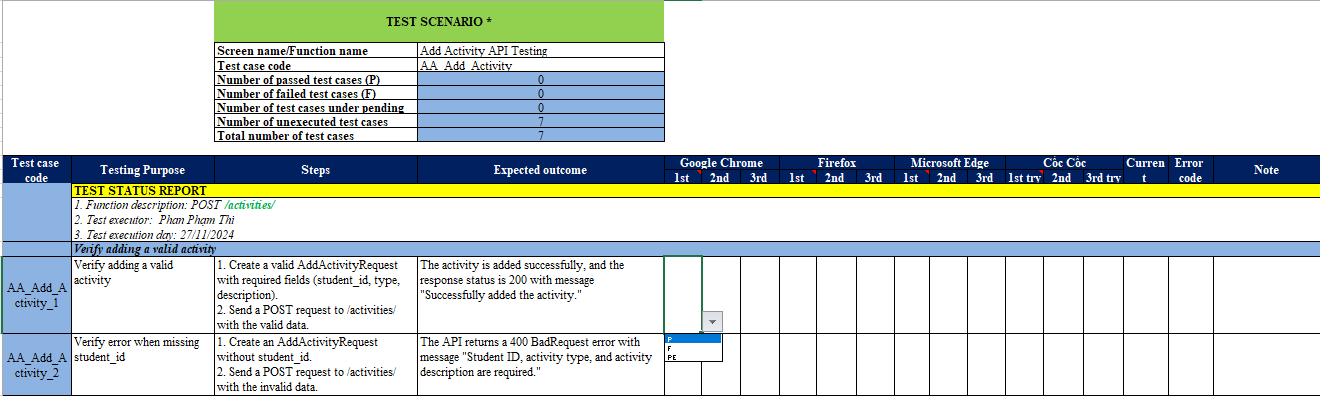
\includegraphics[scale=0.5]{Images/Implement/testScenario.png}
    \caption{Ví dụ về một kịch bản kiểm thử}
\end{figure}
\subsubsection{Mục tiêu của các kịch bản kiểm thử}
\begin{itemize}
    \item \textbf{Kiểm thử chức năng}: Đảm bảo các API hoạt động đúng với các yêu cầu và dữ liệu đầu vào hợp lệ hoặc không hợp lệ. 
    \item \textbf{Kiểm thử tương thích trình duyệt}: Đảm bảo hệ thống hoạt động ổn định trên các trình duyệt phổ biến.
    \item \textbf{Kiểm thử độ tin cậy}: Kiểm tra xem các API có thể xử lý được các tình huống thực tế và đưa ra kết quả chính xác.
\end{itemize}

\section{Các API cần kiểm thử}
Các APIs được kiểm thử sẽ là các APIs có liên quan đến các chức năng chính của hệ thống như:
\begin{itemize}
    \item Sinh ra lộ trình học tập cho sinh viên
    \item Gợi ý mục tiêu học tập cho sinh viên đối với một khóa học cụ thể
    \item Sinh ra bài tập quiz tự động cho sinh viên
    \item Đánh giá kết quả học tập của sinh viên
    \item Tái tạo nội dung bài học cho sinh viên
\end{itemize}

\section{Kết quả kiểm thử API}
\subsection{Kiểm thử phương thức}
% \begin{itemize}
%     \item \textbf{Welcome API Testing}
%     \begin{figure}[H]
%         \centering
%         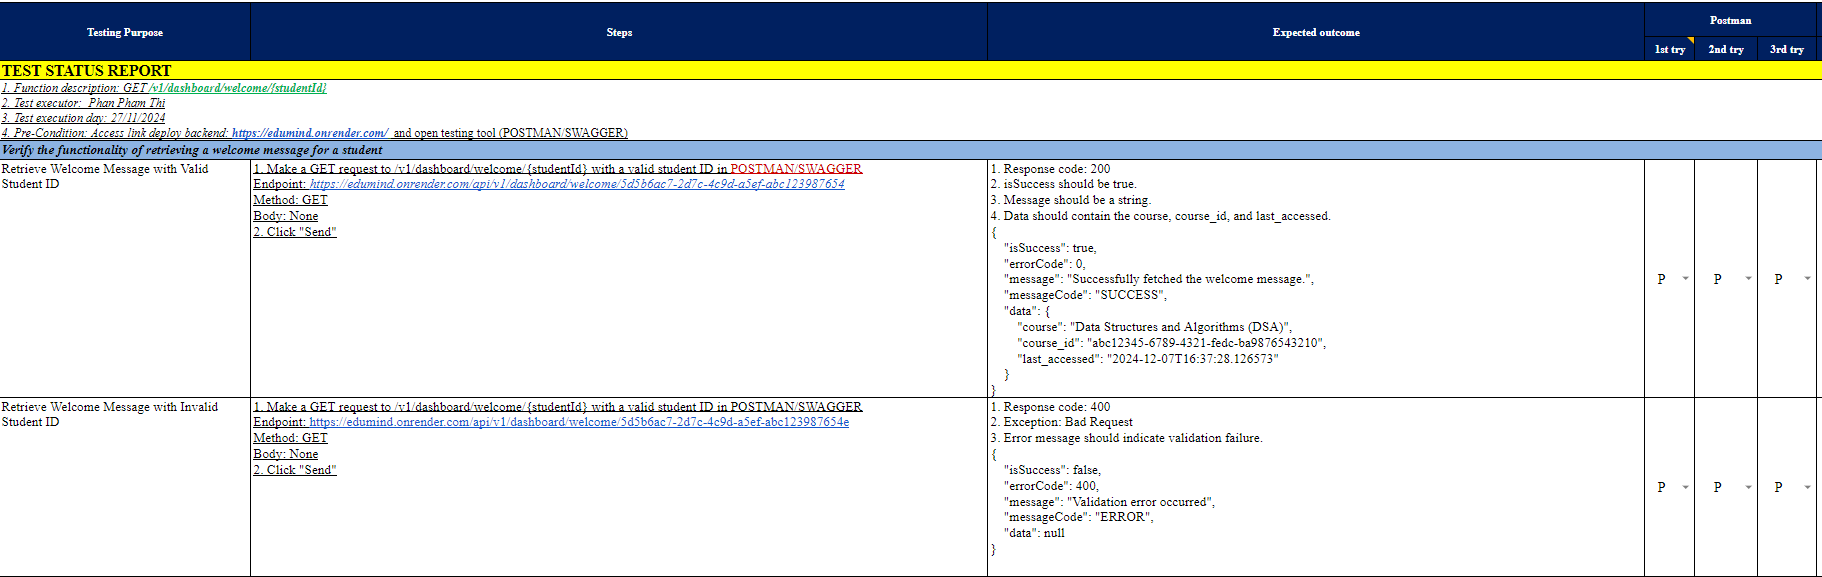
\includegraphics[width=0.8\textwidth]{Images/test/test_WC.png}
%         \caption{Kiểm thử truy xuất các khóa học gần đây}
%     \end{figure}
%     Minh họa cách hệ thống truy xuất thông tin về các khóa học gần đây mà sinh viên đã tham gia hoặc có liên quan.
%     \item \textbf{Get Activities API Testing}
%     \begin{figure}[H]
%         \centering
%         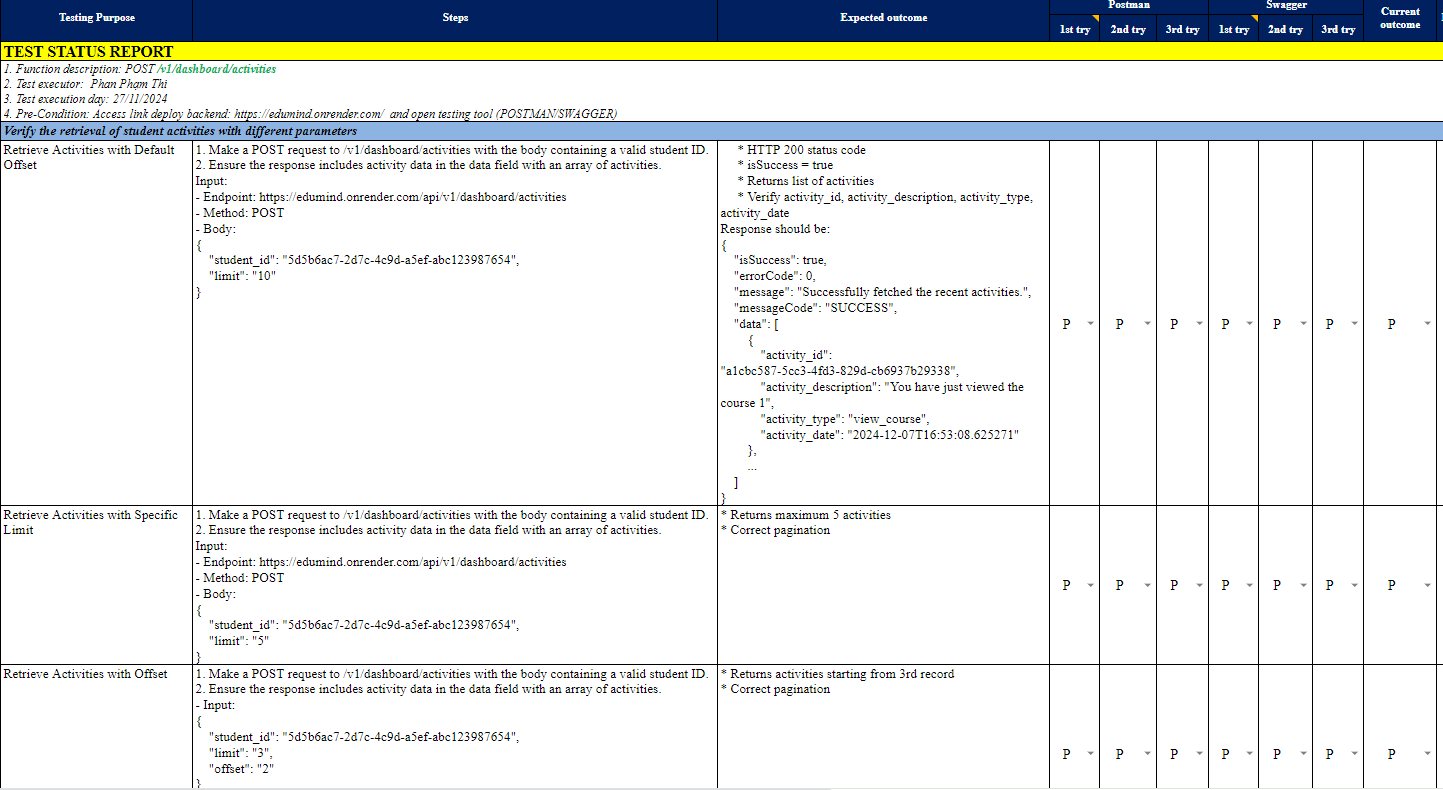
\includegraphics[width=0.8\textwidth]{Images/test/test_GA.png}
%         \caption{Kiểm thử truy xuất các hoạt động gần đây}
%     \end{figure}
%     Hiển thị kết quả kiểm thử cho việc truy xuất các hoạt động gần đây của sinh viên trong hệ thống.
%     \item \textbf{Courses List API Testing}
%     \begin{figure}[H]
%         \centering
%         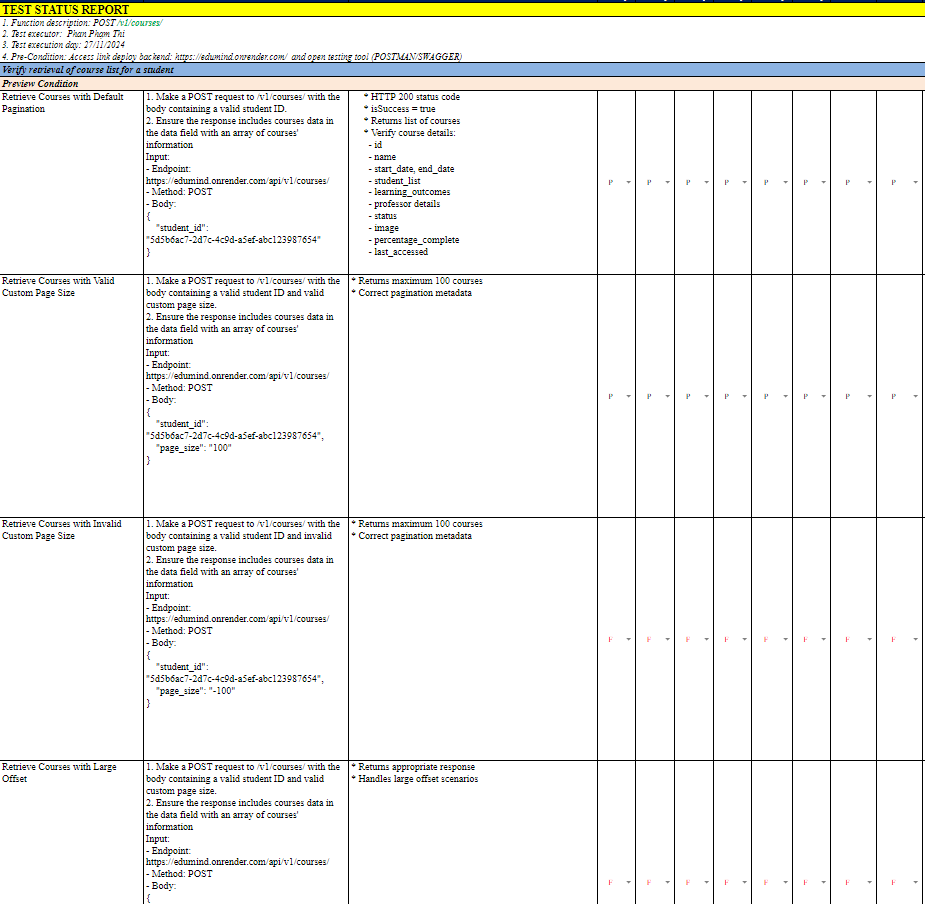
\includegraphics[width=0.8\textwidth]{Images/test/test_CL.png}
%         \caption{Kiểm thử truy xuất danh sách khóa học của sinh viên}
%     \end{figure}
%     Thể hiện chi tiết kết quả khi lấy danh sách các khóa học mà sinh viên đã đăng ký hoặc tham gia.
%     \item \textbf{Get Course for Student API Testing}
%     \begin{figure}[H]
%         \centering
%         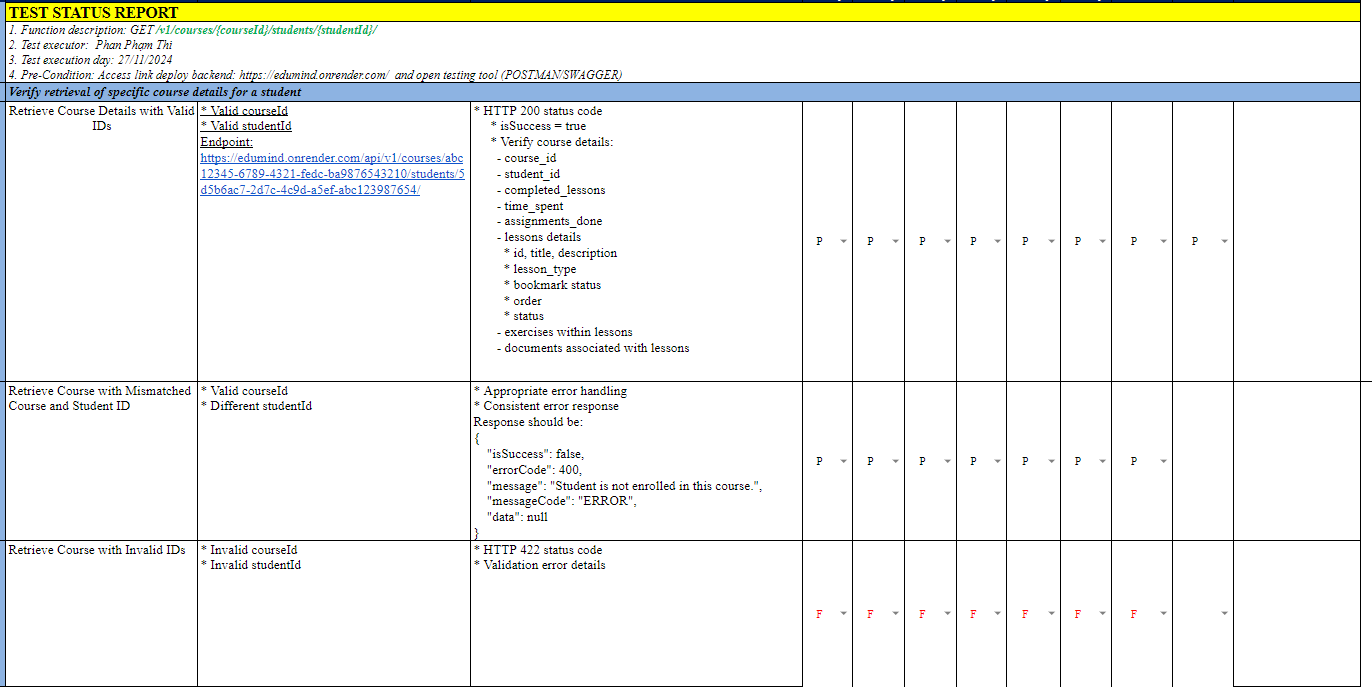
\includegraphics[width=0.8\textwidth]{Images/test/test_CD.png}
%         \caption{Kiểm thử truy xuất chi tiết một khóa học}
%     \end{figure}
%     Kết quả trả về chi tiết thông tin của một khóa học cụ thể trong hệ thống.
%     \item \textbf{Recommended Courses List API Testing}
%     \begin{figure}[H]
%         \centering
%         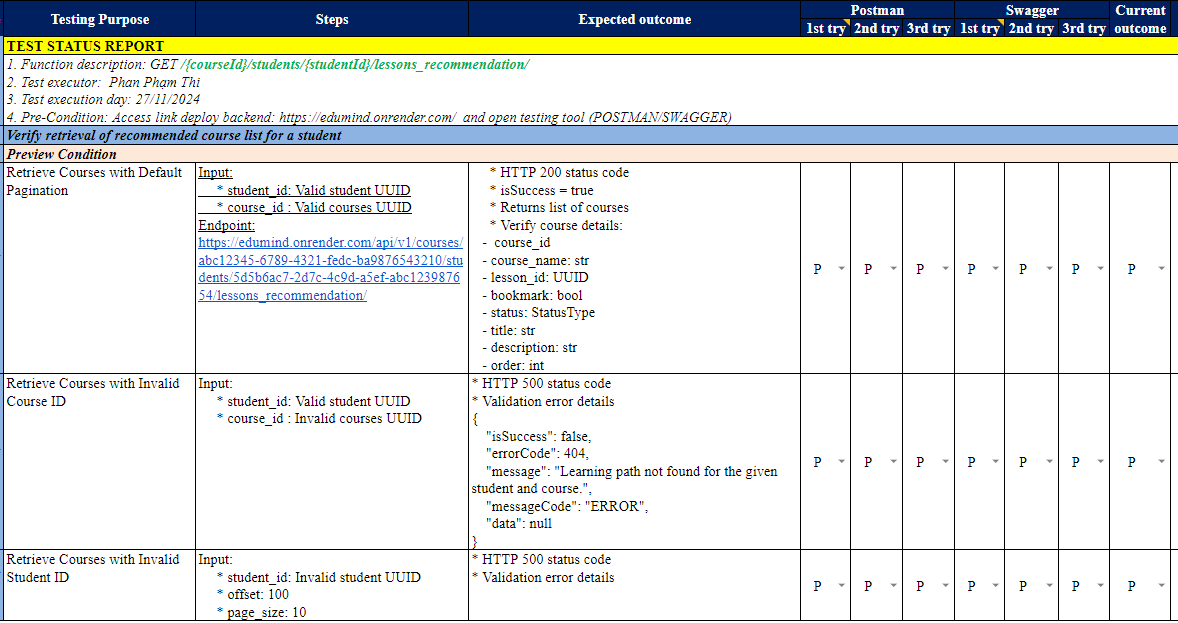
\includegraphics[width=0.8\textwidth]{Images/test/test_RCL.png}
%         \caption{Kiểm thử truy xuất danh sách khóa học được đề xuất}
%     \end{figure}
%     Truy xuất danh sách các khóa học được hệ thống đề xuất dựa trên sở thích hoặc lịch sử học tập của sinh viên.
%     \item \textbf{Add Activity API Testing}
%     \begin{figure}[H]
%         \centering
%         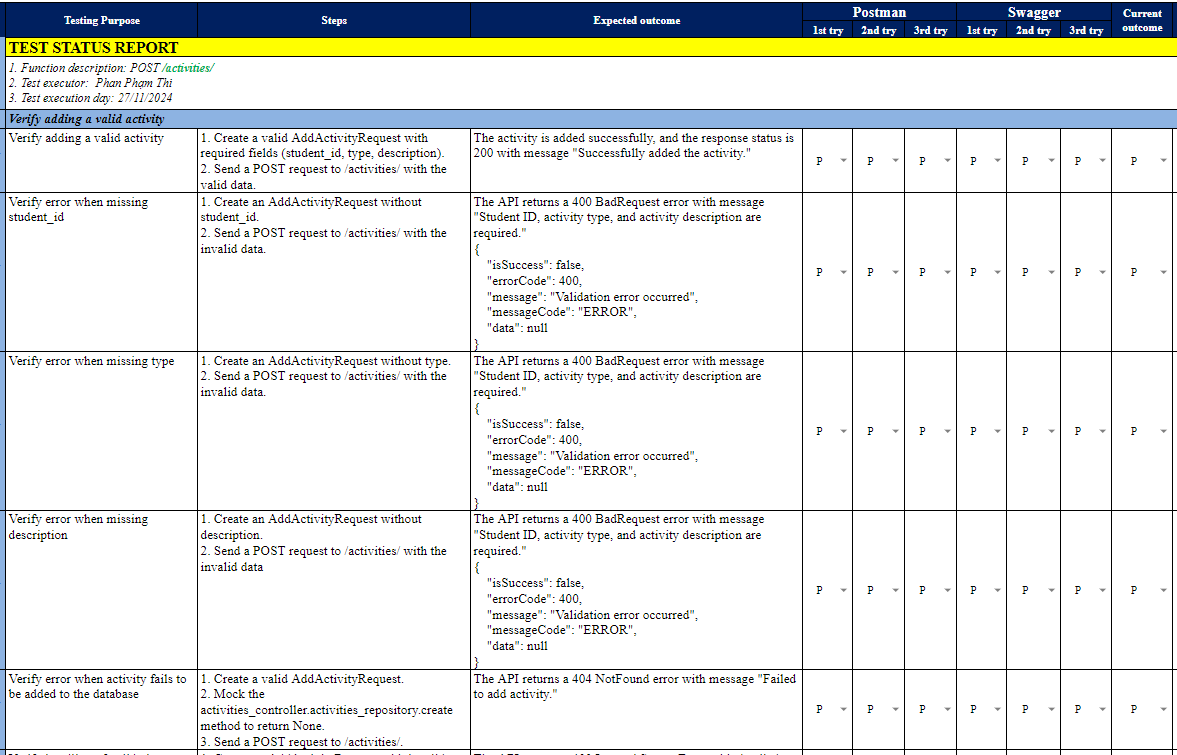
\includegraphics[width=0.8\textwidth]{Images/test/test_AA.png}
%         \caption{Kiểm thử thêm hoạt động gần đây của sinh viên}
%     \end{figure}
%     Minh họa kiểm thử chức năng ghi nhận một hoạt động mới vào danh sách các hoạt động gần đây của sinh viên.
%     \item \textbf{Recommend Lesson API Testing}
%     \begin{figure}[H]
%         \centering
%         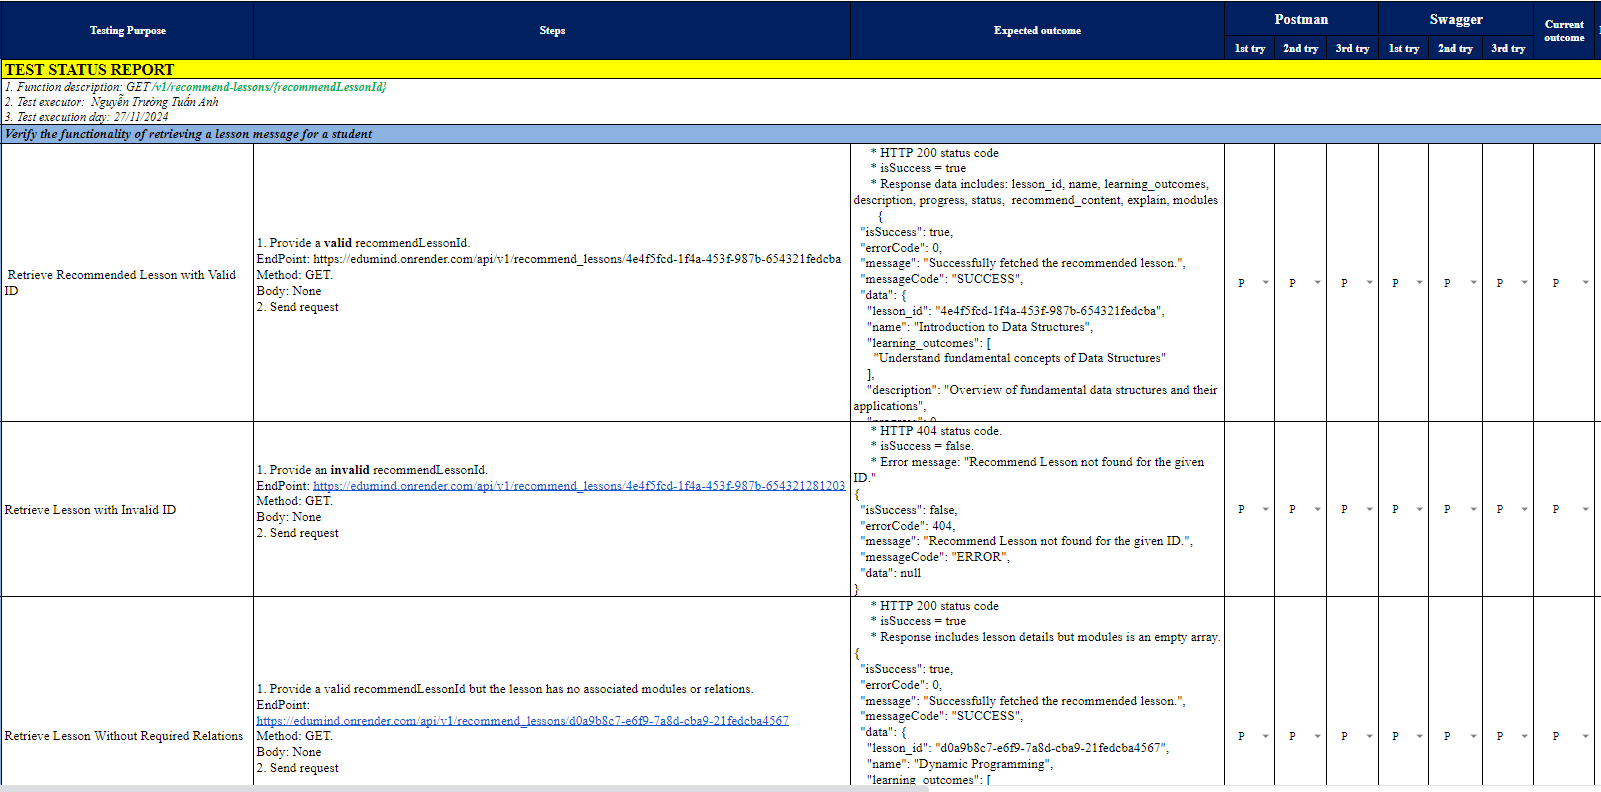
\includegraphics[width=0.8\textwidth]{Images/test/test_RL.png}
%         \caption{Kiểm thử truy xuất chi tiết một lesson được đề xuất}
%     \end{figure}
%     Thể hiện kết quả kiểm thử khi truy xuất chi tiết về một bài học được hệ thống đề xuất.
%     \item \textbf{Quizzes List API Testing}
%     \begin{figure}[H]
%         \centering
%         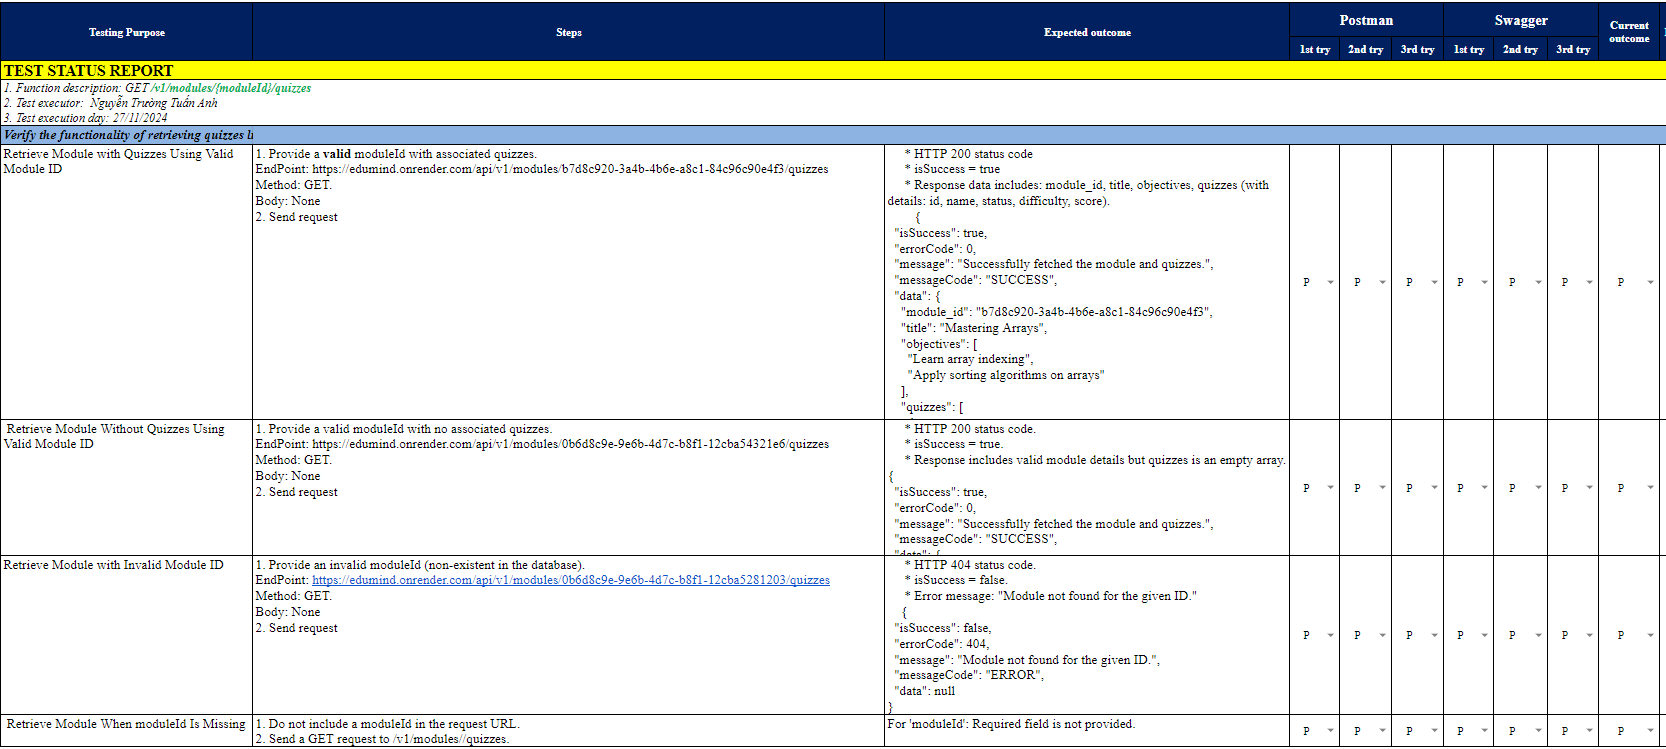
\includegraphics[width=0.8\textwidth]{Images/test/test_QL.png}
%         \caption{Kiểm thử truy xuất danh sách bài tập quizzes từ module}
%     \end{figure}
%     Hiển thị kết quả kiểm thử danh sách bài tập dạng quiz từ một module cụ thể.
%     \item \textbf{Quiz Detail API Testing}
%     \begin{figure}[H]
%         \centering
%         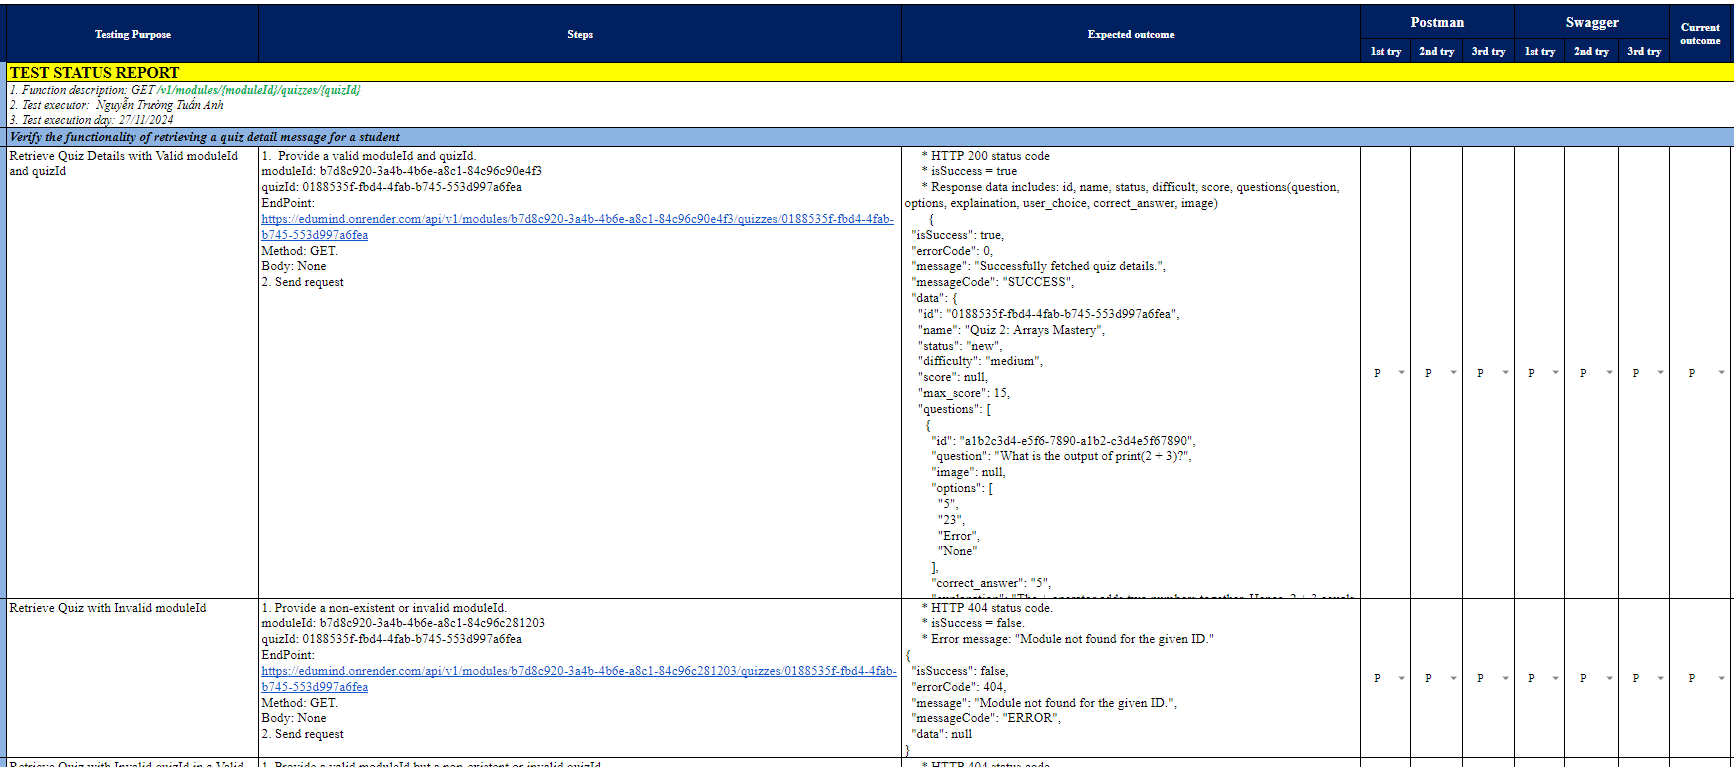
\includegraphics[width=0.8\textwidth]{Images/test/test_DQ.png}
%         \caption{Kiểm thử truy xuất chi tiết một bài tập quiz}
%     \end{figure}
%     Kết quả kiểm thử truy xuất thông tin chi tiết về một bài tập quiz trong danh sách.
%     \item \textbf{Clear Answer API Testing}
%     \begin{figure}[H]
%         \centering
%         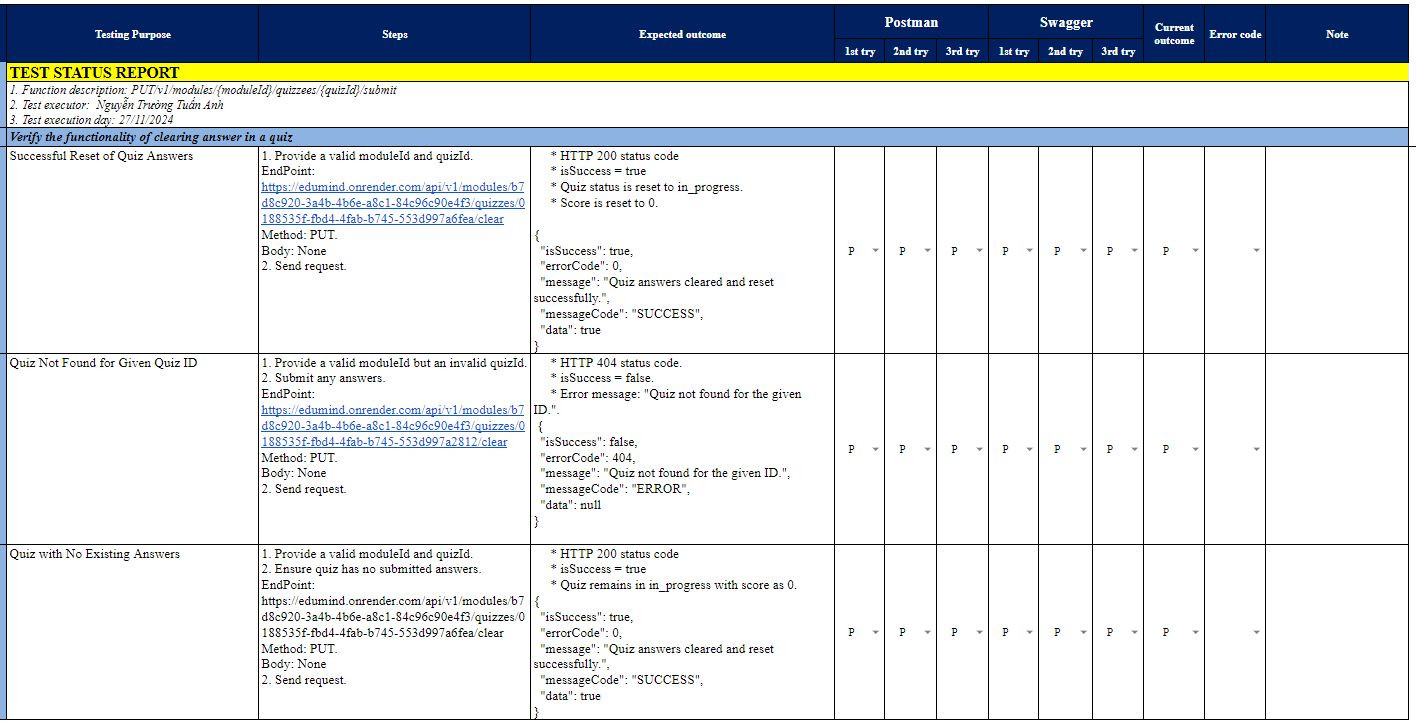
\includegraphics[width=0.8\textwidth]{Images/test/test_CA.png}
%         \caption{Kiểm thử bắt đầu làm lại một bài tập quiz}
%     \end{figure}
%     Thể hiện kết quả thử nghiệm chức năng cho phép sinh viên bắt đầu làm lại một bài tập quiz đã làm trước đó.
%     \item \textbf{Submit Answer API Testing}
%     \begin{figure}[H]
%         \centering
%         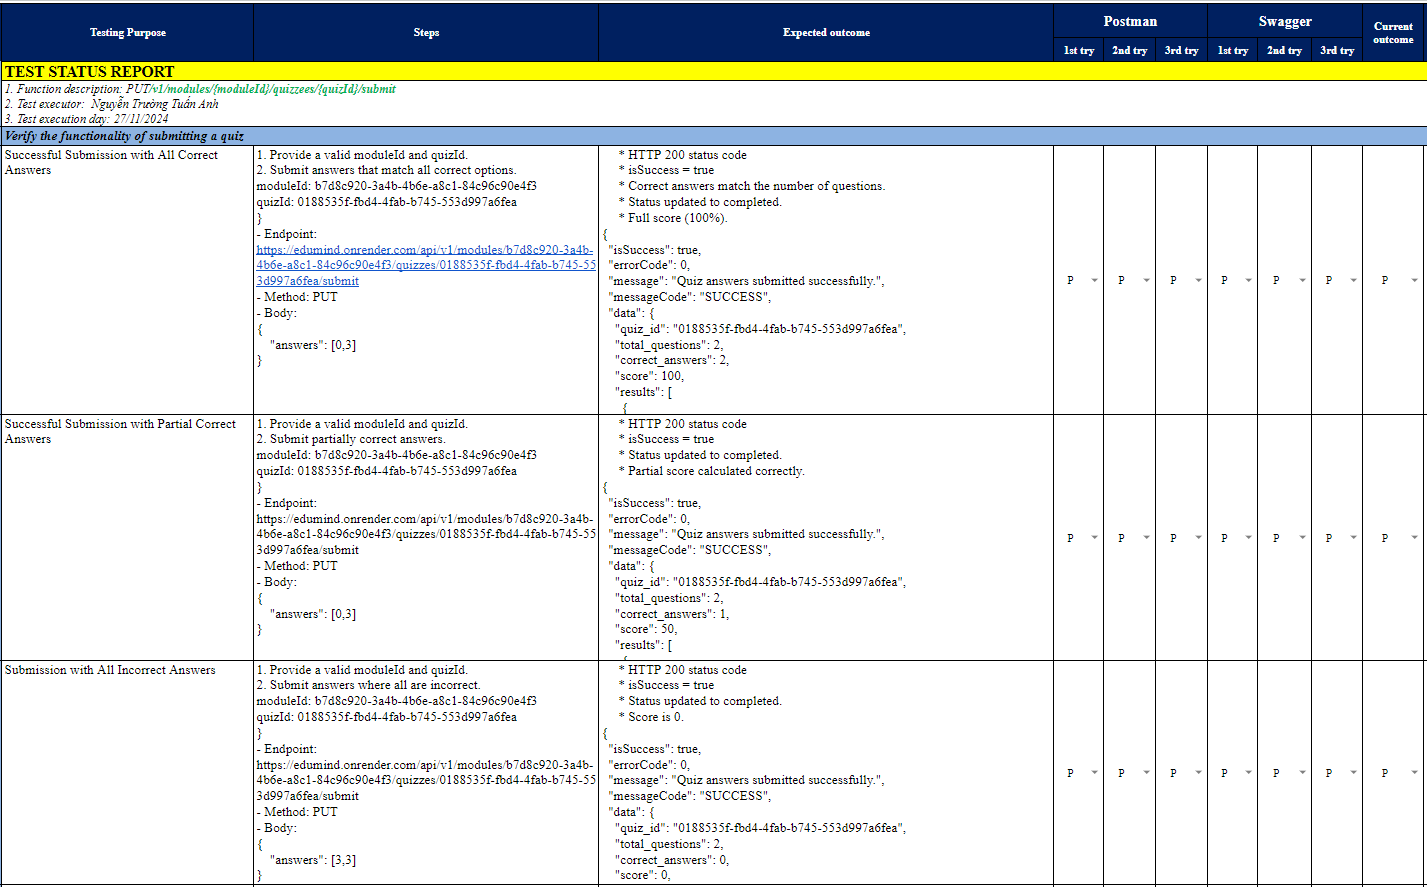
\includegraphics[width=0.8\textwidth]{Images/test/test_SA.png}
%         \caption{Kiểm thử submit một bài tập quiz}
%     \end{figure}
%     Kiểm tra chức năng nộp bài làm cho một bài tập quiz thông qua hệ thống.
%     \item \textbf{Document API Testing}
%     \begin{figure}[H]
%         \centering
%         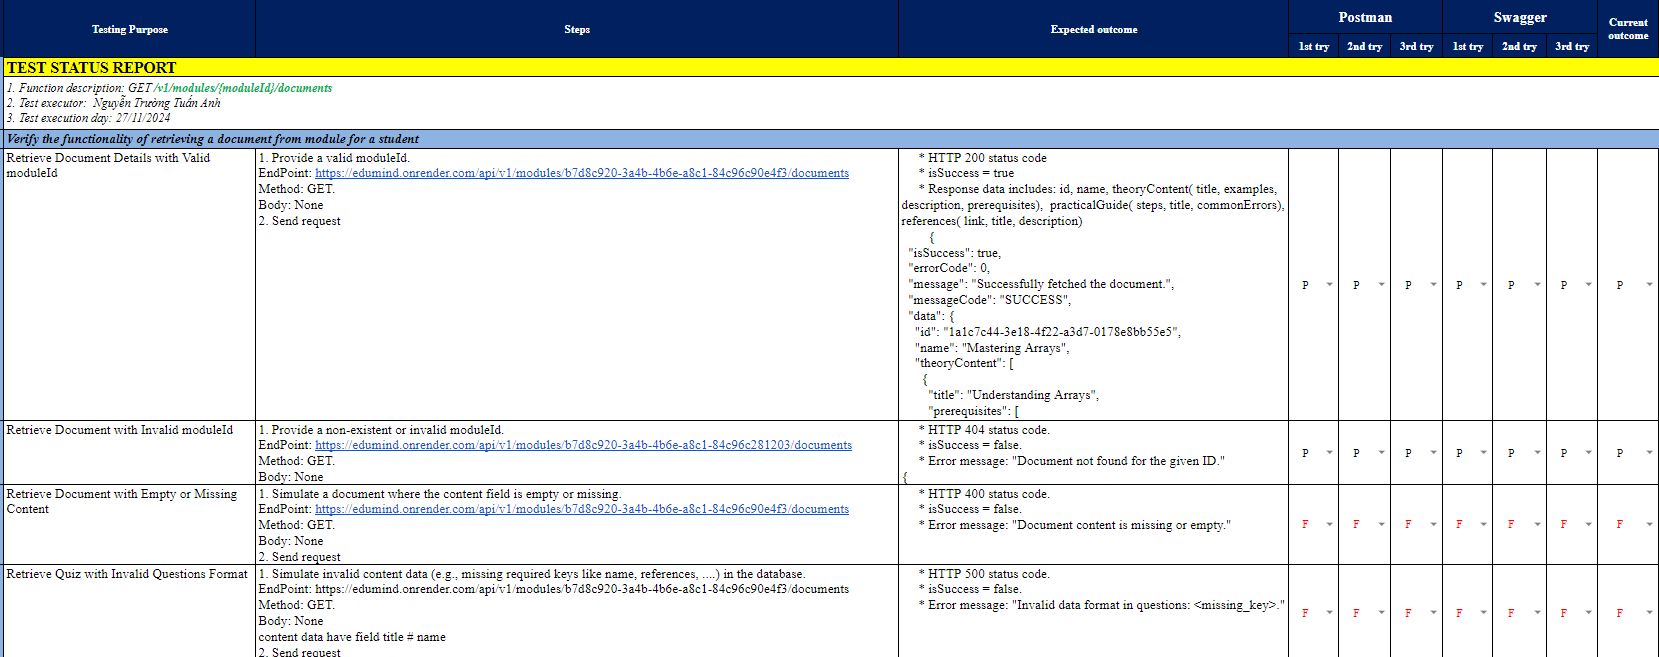
\includegraphics[width=0.8\textwidth]{Images/test/test_DO.png}
%         \caption{Kiểm thử truy xuất document từ module}
%     \end{figure}
%     Minh họa việc truy xuất tệp tài liệu từ một module khóa học.
% \end{itemize}
\subsection{Kết quả tổng hợp của các testcase}
% \begin{figure}[H]
%     \centering
%     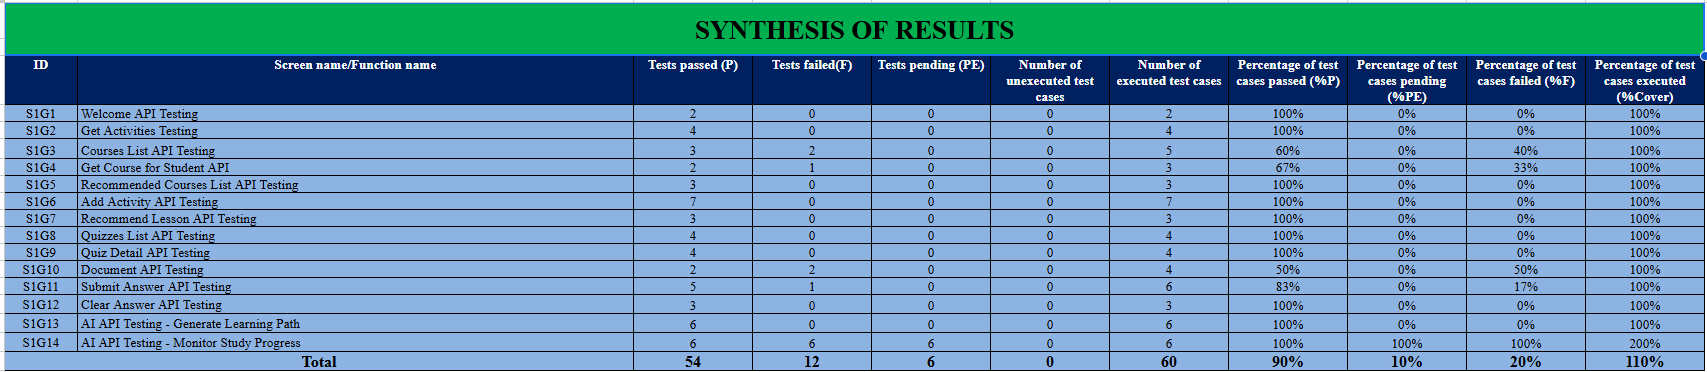
\includegraphics[width=0.8\textwidth]{Images/test/synthesisResults.png}
%     \caption{Kết quả tổng hợp của các testcase}
% \end{figure}
% \begin{itemize}
%     \item Kết quả tổng quan:
%     \begin{itemize}
%         \item \textbf{Số lượng test case đã thực thi:} Toàn bộ 48 test case đã được thực thi, đạt tỷ lệ bao phủ kiểm thử là 100\%.
%         \item \textbf{Số lượng test case đã vượt qua:} Có 42 test case thành công, chiếm 88\% tổng số test case.
%         \item \textbf{Số lượng test case thất bại:} Có 6 test case thất bại, chiếm 13\% tổng số test case.
%         \item \textbf{Số lượng test case đang chờ xử lý:} Không có test case nào đang chờ xử lý (0\%).
%     \end{itemize}
%     \item Phân tích chi tiết theo từng chức năng
%     \begin{itemize}
%         \item \textbf{Welcome API Testing, Get Activities Testing, Recommended Courses List API Testing, Add Activity API Testing, Recommend Lesson API Testing, Quizzes List API Testing, Quiz Detail API Testing, Clear Answer API Testing:} 
%         Các chức năng này đều đạt tỷ lệ thành công 100\%, không có lỗi xảy ra trong quá trình kiểm thử.
        
%         \item \textbf{Courses List API Testing:} Tỷ lệ thành công đạt 60\% với 3 test case vượt qua và 2 test case thất bại.
        
%         \item \textbf{Get Course for Student API:} Tỷ lệ thành công đạt 67\%, với 2 test case vượt qua và 1 test case thất bại.
        
%         \item \textbf{Document API Testing:} Có tỷ lệ thành công thấp nhất (50\%), với 2 test case vượt qua và 2 test case thất bại.
        
%         \item \textbf{Submit Answer API Testing:} Đạt tỷ lệ thành công 83\%, với 5 test case vượt qua và 1 test case thất bại.
%     \end{itemize}
% \end{itemize}

\section{Hạn chế}
% \begin{itemize}
%     \item Do nhóm chưa có nhiều kinh nghiệm trong việc thực hiện unit testing.
%     \item Quá trình kiểm thử chủ yếu tập trung vào kiểm tra chức năng API mà chưa thực hiện đầy đủ các kiểm thử liên quan đến giao diện người dùng (UI testing) hoặc hiệu năng hệ thống (performance testing). 
%     \item Một số API vẫn còn thất bại, đặc biệt là Courses List API Testing và Document API Testing, cần được kiểm tra và sửa lỗi.
% \end{itemize}
